\chapter{Исследовательский раздел}
В данном разделе приведены характеристики используемого устройства, описано проводимое исследование, демонстрируются результаты данного исследования и их анализ.

\section{Технические характеристики}
Технические характеристики используемого устройства:
\begin{itemize}
	\item[---] операционная система --- Ubuntu Linux x86\_64~\cite{Ubuntu};
	\item[---] память --- 16 Гб;
	\item[---] процессор --- AMD Ryzen 5 5500U (6x2.10 ГГц)~\cite{AMD}.
\end{itemize}

\section{Описание исследования}
Целью исследования является проверить зависимость времени выполнения запроса от наличия индексации на различном количестве записей в таблице.

Для проведения исследования была выбрана таблица book\_author, которая служит таблицей-связкой для авторов и книг. Так как необходимо иметь возможность быстро получать все книги определенного автора, то для индексации был выбран столбец author\_id. Замеры проводились на количестве записей от 10 до 2500.

В листинге~\ref{lst:index_1} демонстрируется рассматриваемый запрос, на котором будут проводиться замеры. Значение author\_id берется из таблицы В листинге~\ref{lst:index_2} демонстрируется создание индекса в таблице book\_author.

\begin{center}
	\captionsetup{justification=raggedright,singlelinecheck=off}
	\begin{lstlisting}[language=sql, frame=single, numbers=left, label=lst:index_1, caption=Рассматриваемый запрос]
SELECT b.*
FROM book_author ba
JOIN book b ON ba.book_id = b.id
WHERE ba.author_id = author_id;
	\end{lstlisting}
\end{center}


\begin{center}
	\captionsetup{justification=raggedright,singlelinecheck=off}
	\begin{lstlisting}[language=sql, frame=single, numbers=left, label=lst:index_2, caption=Создание роли модератора]
CREATE INDEX idx_book_author_author_id ON book_author(author_id);
	\end{lstlisting}
\end{center}

\section{Результаты исследования}

В таблице~\ref{tbl:time} приведены результаты исследования. Для каждого размера было проведено 1000 замеров, значение в таблице взято как среднее арифметическое от них.

\begin{table}[H]
	\begin{center}
		\caption{Результаты исследования}
		\begin{tabular}{|l|l|l|}
			\hline
			\textbf{Количество записей} & \textbf{Без индекса, мс} & \textbf{С индексом, мс} \\
			\hline
			10 & 0.017 & 0.01145 \\
			\hline
			30 & 0.018 & 0.01150 \\
			\hline
			60 & 0.021 & 0.01151 \\
			\hline
			100 & 0.022 & 0.01152 \\
			\hline
			300 & 0.040 & 0.01153 \\
			\hline
			600 & 0.057 & 0.01142 \\
			\hline
			1000 & 0.066 & 0.01149 \\
			\hline
			1500 & 0.092 & 0.01140 \\
			\hline
			2000 & 0.105 & 0.01151 \\
			\hline
			2500 & 0.129 & 0.01154 \\
			\hline
		\end{tabular}
		\label{tbl:time}
	\end{center}
\end{table}

\clearpage
Графическая интерпретация результатов представлена на рисунке~\ref{fig:graph}.

\begin{figure}[H]
	\centering
	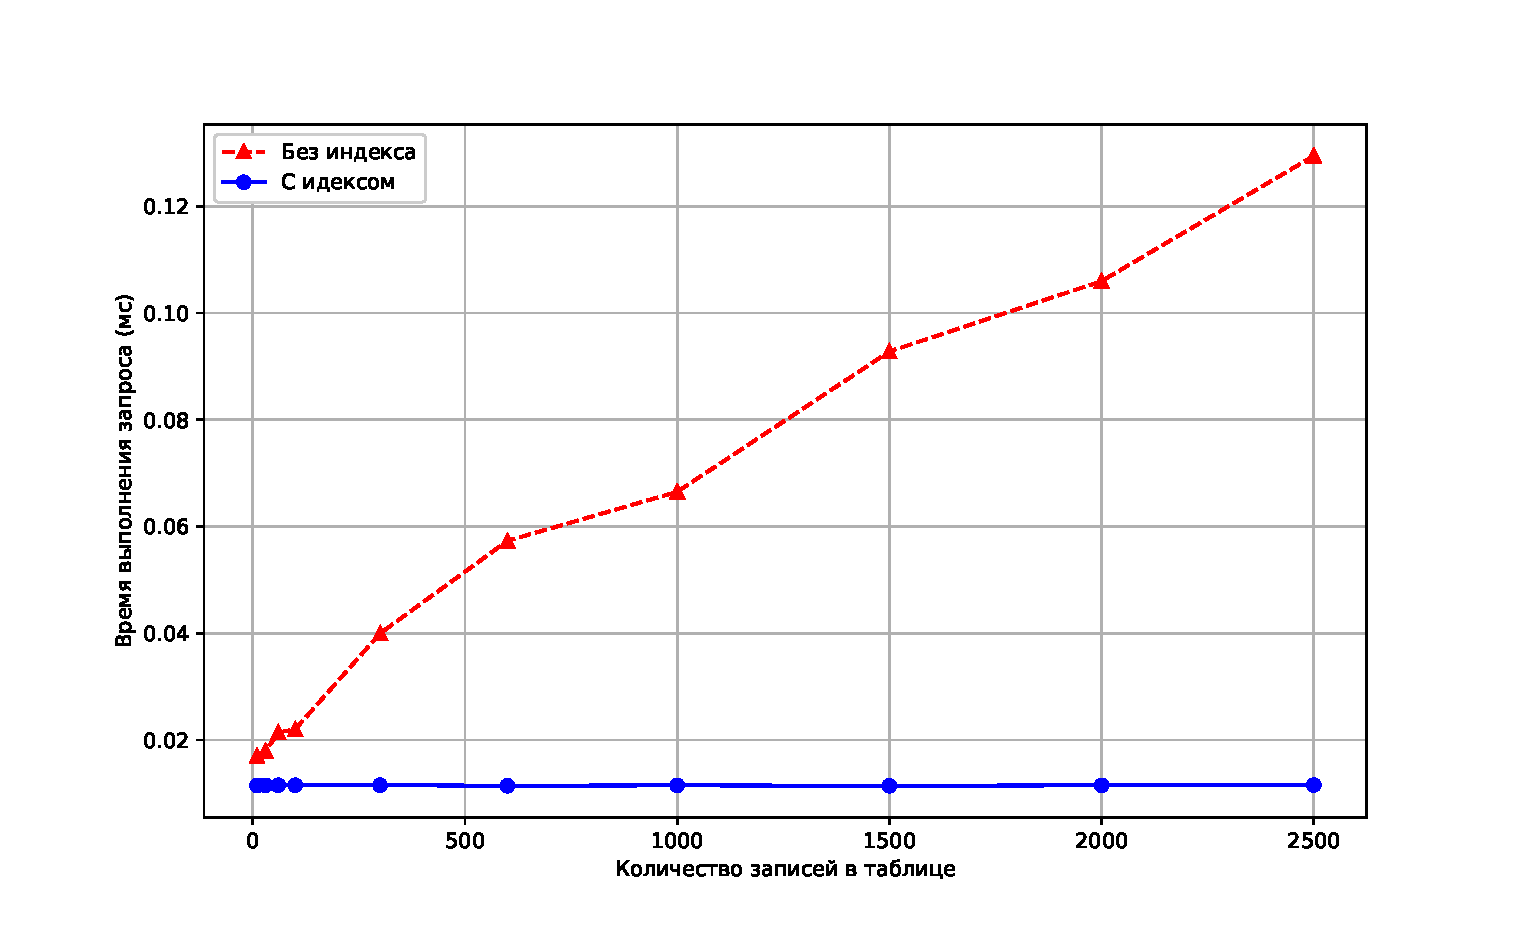
\includegraphics[scale=0.7]{img/graph.eps}
	\caption{Зависимость времени выполнения запроса от количества записей в таблице}
	\label{fig:graph}
\end{figure}

Из полученных результатов видно, что наличие индексации в базе данных дает выигрыш по времени даже при 10 записях, тогда как при 100 время выполнения запроса с индексом сокращается приблизительно в 2 раза. При 2500 записей время выполнения запроса сокращается более чем в 10 раз. 
Также из полученных данных следует, что время выполнения запроса без индекса с увеличением количества записей возрастает, тогда как время выполнения запроса с индексом остается приблизительно одинаковым.

\clearpage
\textbf{ВЫВОД}

В данном разделе были рассмотрены технические характеристики устройства, было описано исследование зависимости скорости выполнения запроса от наличия индексации на разном количестве записей в базе данных. 

Результаты показали, что в отсутствие индекса время выполнения запроса увеличивается по мере роста числа записей, тогда как при наличии индекса оно остается практически неизменным. Причем даже при малом объеме данных запрос без индекса выполняется дольше: при 100 записях --- приблизительно в два раза медленнее, при 2500 --- более чем в десять раз.

\clearpage